\section{Задача 1.26}
\subsection{Задание:}
Решить систему линейных уравнений методом Крамера в компьютерной среде
\\[1em]
$
	\begin{cases}
		3x_1 + 2x_2 + x_3 = 5  \\
		2x_1 + 3x_2 + x_3 = 1  \\
		2x_1 + x_2 + 3x_3 = 11 \\
	\end{cases}
$
\subsection{Решение:}
Решим СЛУ в системе Wolfram Mathematica:
Найдём $ \Delta $:
\\
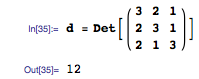
\includegraphics[scale=0.6]{task/1_26/screen1.png}
\\
Найдём $ \Delta_1, \Delta_2, \Delta_3 $:
\\
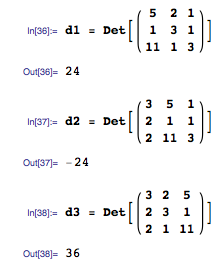
\includegraphics[scale=0.6]{task/1_26/screen2.png}
\\
Найдём корни уравнения:
\\
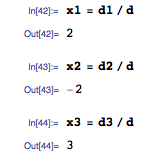
\includegraphics[scale=0.6]{task/1_26/screen3.png}
\\
\subsection{Вывод:}
Мы нашли решение системы методом Крамера: $ x_1 = 2, x_2 = -2, x_3 = 3 $.
